\documentclass[a4paper,20pt]{article}
\usepackage{amsmath,amssymb,epsf,epsfig,times}
\usepackage{multicol}
\usepackage[all]{xy}
\usepackage{color}
\usepackage{ctex}
\usepackage{subfigure}
\usepackage{url,cite}
\usepackage{tikz}
\usepackage[english]{babel}
\usepackage[utf8]{inputenc}

\usepackage{pdfpages}

%\usepackage{caption}
%
%\usepackage[font=small,labelfont=bf,labelsep=none]{caption}
\usepackage[font=default,labelfont=bf,labelsep=period]{caption}

\usepackage{makecell}
\usepackage{booktabs} %引入三线表
\usepackage{diagbox}
\usepackage{multirow}

\usepackage{fancyhdr}
\usepackage{float}
\usepackage{ulem}

\usepackage{listings}
\usepackage{xcolor}

\usepackage{enumerate}
\lstset{
    basicstyle          =   \sffamily,          % 基本代码风格
    keywordstyle        =   \bfseries,          % 关键字风格
    commentstyle        =   \rmfamily\itshape,  % 注释的风格,斜体
    stringstyle         =   \ttfamily,  % 字符串风格
    flexiblecolumns,                % 别问为什么,加上这个
    numbers             =   left,   % 行号的位置在左边
    showspaces          =   false,  % 是否显示空格,显示了有点乱,所以不现实了
    numberstyle         =   \zihao{-5}\ttfamily,    % 行号的样式,小五号,tt等宽字体
    showstringspaces    =   false,
    captionpos          =   t,      % 这段代码的名字所呈现的位置,t指的是top上面
    frame               =   lrtb,   % 显示边框
}
\lstdefinestyle{Python}{
    language        =   Python, % 语言选Python
    basicstyle      =   \zihao{-5}\ttfamily,
    numberstyle     =   \zihao{-5}\ttfamily,
    keywordstyle    =   \color{blue},
    keywordstyle    =   [2] \color{teal},
    stringstyle     =   \color{magenta},
    commentstyle    =   \color{red}\ttfamily,
    breaklines      =   true,   % 自动换行,建议不要写太长的行
    columns         =   fixed,  % 如果不加这一句,字间距就不固定,很丑,必须加
    basewidth       =   0.5em,
}

\newtheorem{theorem}{Theorem}[section]
\newtheorem{lemma}{Lemma}[section]
\def\proof{\noindent{\it Proof: }}
\def\QED{\mbox{\rule[0pt]{1.5ex}{1.5ex}}}
\def\endproof{\hspace*{\fill}~\QED\par\endtrivlist\unskip}
\newcommand{\re}{\mathbb{R}}
\def\sV{\mathcal{V}}
\def\sS{\mathcal{S}}
\def\sQ{\mathcal{Q}}

\newcommand{\mc}{\mbox{: }}

\newcommand{\normsq}[1]{\left\|#1\right\|^2}
\newcommand{\norm}[1]{\left\|#1\right\|}
%\newcommand{\sgn}[1]{\mbox{sgn}(#1)}
\newcommand{\pde}[2]{\frac{\partial #1}{\partial #2}}
\newcommand{\fundef}[3]{#1:#2\to #3}
\newcommand{\abs}[1]{\left|#1\right|}
\newcommand{\mymatrix}[2]{\left(\begin{array}{#1}#2\end{array}\right)}
\newcommand{\defeq}{\stackrel{\triangle}{=}}
\newcommand{\paren}[1]{\left(#1\right)}
%\theoremstyle{plain} \newtheorem{theorem}{Theorem}
%\theoremstyle{plain} \newtheorem{algorithm}{Algorithm}
\newtheorem{axiom}[theorem]{Axiom}
\newtheorem{definition}[theorem]{Definition}
\newtheorem{assumption}[theorem]{Assumption}
\newtheorem{example}[theorem]{Example}
%\theoremstyle{plain}\newtheorem{lemma}{Lemma}
%\newtheorem{proposition}[theorem]{Proposition}
\newtheorem{remark}[theorem]{Remark}
\newtheorem{corollary}[theorem]{Corollary}

\newcommand{\Acal}{\mathcal{A}}
\newcommand{\Bcal}{\mathcal{B}}
\newcommand{\Ccal}{\mathcal{C}}
\newcommand{\Dcal}{\mathcal{D}}
\newcommand{\Ecal}{\mathcal{E}}
\newcommand{\Fcal}{\mathcal{F}}
\newcommand{\Gcal}{\mathcal{G}}
\newcommand{\Hcal}{\mathcal{H}}
\newcommand{\Ical}{\mathcal{I}}
\newcommand{\Jcal}{\mathcal{J}}
\newcommand{\Kcal}{\mathcal{K}}
\newcommand{\Lcal}{\mathcal{L}}
\newcommand{\Mcal}{\mathcal{M}}
\newcommand{\Ncal}{\mathcal{N}}
\newcommand{\Ocal}{\mathcal{O}}
\newcommand{\Pcal}{\mathcal{P}}
\newcommand{\Qcal}{\mathcal{Q}}
\newcommand{\Rcal}{\mathcal{R}}
\newcommand{\Scal}{\mathcal{S}}
\newcommand{\Tcal}{\mathcal{T}}
\newcommand{\Ucal}{\mathcal{U}}
\newcommand{\Vcal}{\mathcal{V}}
\newcommand{\Wcal}{\mathcal{W}}
\newcommand{\Xcal}{\mathcal{X}}
\newcommand{\Ycal}{\mathcal{Y}}
\newcommand{\Zcal}{\mathcal{Z}}


\def\omegavec{\boldsymbol{\omega}}
\newcommand{\alphabf}{\boldsymbol{\alpha}}
\newcommand{\omegabf}{\boldsymbol{\omega}}
\def\omegavec{\boldsymbol{\omega}}
\newcommand{\taubf}{\boldsymbol{\tau}}
\newcommand{\qbf}{\mathbf{q}}
\newcommand{\ybf}{\mathbf{y}}
\newcommand{\pbf}{\mathbf{p}}
\newcommand{\rbf}{\mathbf{r}}
\newcommand{\ebf}{\mathbf{e}}
\newcommand{\onebf}{\mathbf{1}}
\newcommand{\zerobf}{\mathbf{0}}
\newcommand{\abf}{\mathbf{a}}
\newcommand{\ibf}{\mathbf{i}}
\newcommand{\jbf}{\mathbf{j}}
\newcommand{\kbf}{\mathbf{k}}
\newcommand{\vbf}{\mathbf{v}}
\newcommand{\wbf}{\mathbf{\omega}}
\newcommand{\fbf}{\mathbf{f}}
\newcommand{\zbf}{\mathbf{z}}
\newcommand{\xbf}{\mathbf{x}}
\newcommand{\dbf}{\mathbf{d}}
\newcommand{\Rbf}{\mathbf{R}}
\newcommand{\Tbf}{\mathbf{T}}

\newcommand{\Cbf}{\mathbf{C}}
\newcommand{\Ibf}{\mathbf{I}}
\newcommand{\Pbf}{\mathbf{P}}
\newcommand{\Qbf}{\mathbf{Q}}
\newcommand{\Vbf}{\mathbf{V}}
\newcommand{\Jbf}{\mathbf{J}}
\newcommand{\Xbf}{\mathbf{X}}
\newcommand{\Abf}{\mathbf{A}}
\newcommand{\Kbf}{\mathbf{K}}
\newcommand{\Gammabf}{\boldsymbol{\Gamma}}
\newcommand{\nubf}{\boldsymbol{\nu}}
\newcommand{\xibf}{\boldsymbol{\xi}}
\newcommand{\Xibf}{\boldsymbol{\Xi}}
\newcommand{\Omegabf}{\boldsymbol{\Omega}}


\newcommand{\ubf}{\mathbf{u}}

\newcommand{\lth}{\ell{\text{th}}}
\newcommand{\ith}{i{\text{th}}}
\newcommand{\jth}{j{\text{th}}}
\newcommand{\kth}{k{\text{th}}}
\newcommand{\ip}[2]{\left<#1,~#2\right>}

\newcommand{\OMIT}[1]{}
\title{}
\author{}
\date{}


\pagestyle{fancy}
\fancyhf{}
\chead{\textbf{关于$\lceil$\textcolor{red}{“非线性规划”}$\rfloor$的matlab讲解}}
\lhead{魔力铠甲}
\rfoot{Page \thepage}
\begin{document}
\renewcommand{\lstlistlistingname}{代码汇总}
\renewcommand{\lstlistingname}{代码}
\captionsetup[figure]{labelfont={bf},labelformat={default},labelsep=period,name={图}}
\renewcommand\tablename{表}
好的,我们来到了规划类问题的最后一章,动态规划。其实说是最后一章,倒不如说这是对前面三章规划的总结融合,采用最适合的解法去
解决规划问题。
\section{动态规划-简介}
动态规划(Dynamic Programming)是求解某类问题的一种方法,是考察问题的一种途径,而不是
一种特殊算法(如线性规划是一种算法)。动态规划是一种通过将复杂问题分解为一组更简单的子问题来解决复杂问题的方法。
\par \textbf{\textcolor{black}{八股文:}}动态规划是运筹学的一个分支,通常用来解决多阶段决策过程最优化问题。动态规划的基本想法就是将原来的原问题转换为一系列互相联系的子问题,然后通过逐层地推来求得最后的解。
目前,动态规划常常出现在算法竞赛或者笔试面试中,在数学建模中应用较少。

\subsection{已知的结果下,简单的解法}
某厂为扩大生产能力,拟订购某成套4-6套,以分配给其所管辖的1,2,3个分厂使用。预计各分厂分得不同套数的设备后,每年创造的利润(万元)如下表所示。该厂应订购几套设备并如何分配,才能使每年预计创造利润总额最大?
\begin{center}
    \begin{table}[h]
        \caption{不同分厂套数产生利润}
        \begin{tabular}{|c|c|c|c|c|c|c|c|}
            \hline
            \diagbox{分厂}{利润}{套数} & 0套 & 1套 & 2套 & 3套 & 4套 & 5套 & 6套 \\
            \hline
            1                          & 0   & 3   & 5   & 6   & 7   & 6   & 5   \\
            \hline
            2                          & 0   & 4   & 6   & 7   & 8   & 9   & 10  \\
            \hline
            3                          & 0   & 2   & 5   & 9   & 8   & 8   & 7   \\
            \hline
        \end{tabular}
    \end{table}
\end{center}
\par \small{解:} \\
\fbox{%
    \parbox{\textwidth}{%
        \begin{center}

            目标函数 $\max f(x) = \sum\limits_{i=1}^{m}\sum\limits_{j=1}^{n}c_{ij}x_{ij}$
            \\其中$x_{ij}=\left\{\begin{matrix}
                    0 & (x_i\neq j\mbox{套}) \\
                    1 & (x_i=j\mbox{套})     \\
                \end{matrix}\right.$
            \\同时给出约束条件
            \\s.t.$\left\{\begin{matrix}
                    \sum\limits_{i=0}^{m}\sum\limits_{j=0}^{n}x_{ij}=3 \\
                    \mbox{总套数不超过4-6套}                           \\
                \end{matrix}\right.$
        \end{center}

    }%
}
\section{动态规划-适用题目}

\subsection{动态规划适用的赛题:}
最常见的题目大概就是贪心算法一类问题,主要包括最短路径,背包问题,硬币问题,
\par 动态规划问世以来,在经济管理、生产调度、工程技术和最优控制等方面得到了广泛的应用。例如最短路线、库存管理、资源分配、设备更新、排序、装载等问题,用动态规划方法比用其它方法求解更为方便。虽然动态规划主要用于求解以时间划分阶段的动态过程的优化问题,但是一些与时间无关的静态规划(如线性规划、非线性规划),只要人为地引进时间因素,把它视为多阶段决策过程,也可以用动态规划方法方便地求解。
\subsection{模型假设}
1.~ 工厂产品生产示例1:
\par \noindent \fbox{
    \parbox{\textwidth}{
        设某工厂有 1000 台机器,生产两种产品 A、B ,若投入 x 台机器生产 A 产
        品,则纯收入为5x ,若投入 y 台机器生产 B 种产品,则纯收入为4y ,又知:生产 A 种
        产品机器的年折损率为 20\%,生产 B 产品机器的年折损率为 10\%,问在 5 年内如何安
        排各年度的生产计划,才能使总收入最高?       }
}
\par \noindent \textbf{解:}
\begin{center}
    \begin{lstlisting}[caption={Example1},language=Matlab]
        %This is functionk.m
function [max, uk]=functionk(k_Add_1_xk,k)
% k_Add_1_xk=518.4;
% k=5;
    if k == 6
        par_u = 1;
        par_x = 4;
    else
        par_u = 1 - k_Add_1_xk * 0.1;
        par_x = 4 + k_Add_1_xk * 0.9;
    end
        [max, uk]= maxvalue(par_u, par_x)
end
        %This is maxvalue.m
function [par,key]=maxvalue(par_u, par_x)
    if par_u>=0
        par=par_u+par_x;
        key=1;
    else
        par=par_x;
        key=0;
    end
end
        %This is Example1.m
clc
clear
k_Add_1_xk = 0;
max = 0;
uk = [];
for i = [6:-1:1];
    [k_Add_1_xk, u_k] = functionk(k_Add_1_xk, i);
    uk=[uk u_k];
end
uk=flip(uk);
maxprofit = k_Add_1_xk*1000;
x = 1000; 
x_last = 0;
x_last = x;
number=[x_last];
for i = 2:5
    x = 0.9 * x - 0.1 * uk(i) * x_last;
    x_last = x;
    number=[number x_last];
end
disp('The number of intact machines from the first year is:');
number
disp(strcat('maxvalue is ',num2str(maxprofit)))
%The number of intact machines from the first year is:
%number =   1.0e+03 *
%    1.0000    0.9000    0.8100    0.6480    0.5184
%The maxvalue is 19733.8
    \end{lstlisting}
\end{center}
2.~最短路径寻找示例2:
\par \noindent \fbox{
    \parbox{\textwidth}{
        下图是一个线路网, 连线上的数字表示两点之间的距离(或费用)。试寻求一条由 A到G 距离最短(或费用最省)的路线。      }
}
\par 这种题的解法是较为类似的,我们可以直接套用模板。该模板可以适用于无约束的最短路径这一类问题。
求解步骤:
\\( i)将过程划分成恰当的阶段。
\\( ii)正确选择状态变量 xk ,使它既能描述过程的状态,又满足无后效性,同时确定允许状态集合 Xk 。
\\( iii)选择决策变量uk ,确定允许决策集合Uk (xk ) 。
\\( iv)写出状态转移方程。
\\( v)确定阶段指标 vk (xk ,uk ) 及指标函数Vkn 的形式(阶段指标之和,阶段指标之积,阶段指标之极大或极小等)。
\\( vi)写出基本方程即最优值函数满足的递归方程,以及端点条件。
\begin{center}
    \begin{figure}[h]
        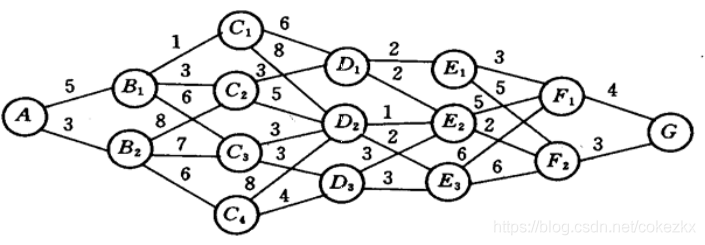
\includegraphics[width=340pt,height=200pt]{figure1.png}
        \caption{示例2}
    \end{figure}
\end{center}
\par \noindent \textbf{解:}
\begin{center}
    \begin{lstlisting}[caption={Example2},language=Matlab]
        % This is Example2.m 
clc,clear 
now=[5,3,0,0 ,0,0,0,0 ,0,0,0,0 ,0,0,0,0 
     1,3,6,0 ,0,8,7,6 ,0,0,0,0 ,0,0,0,0 
     6,8,0,0 ,3,5,0,0 ,0,0,0,0 ,0,0,0,0 
     2,2,0,0 ,1,2,0,0 ,3,3,0,0 ,0,0,0,0 
     3,5,0,0 ,5,2,0,0 ,6,6,0,0 ,0,0,0,0 
     4,0,0,0 ,3,0,0,0 ,0,0,0,0 ,0,0,0,0 
     0,0,0,0 ,0,0,0,0 ,0,0,0,0 ,0,0,0,0]; 
% Distance matrix, the i-th row represents the i-th stage 
% (the last stage is all zeros); 
% n*m columns, n starting points, 
%m different choices, next starting point starts after m numbers 
h=7 ;        
% Number of stages 
a=4   ;      
% Number of starting points 
b=4;         
% Number of decisions (usually equal to the number of starting points) 
% Only need to modify the code above %
% to nest it into other shortest path calculations %
  
  
now(now==0)=inf;    
% First, convert it into a full matrix, use 00 to represent no route,
% then convert 0 to infinity 
road_sum=zeros(h,a*b);   
% Save the shortest distance of each stage 
  
for i=h-1:-1:1      
% Different stages 
    for n=1:a       
    % Different starting points in each stage 
        for k=1:b   
        % Different decisions in each starting point 
road_sum(i,(n-1)*a+k)=now(i,(n-1)*a+k)+min(road_sum(i+1,(k-1)*a+1:k*a));   
% Current path plus the shortest path in the previous stage 
        end 
    end 
end 
  
road=[];                
% Used to save the selected starting points 
for i=1:h-1 
    if i==1 
        start=find(road_sum(1,:)==min(road_sum(1,:)));       
% Find the first point after the starting point 
    else 
start=find(road_sum(i,(start-1)*a+1:start*a)==min(road_sum(i,(start-1)*a+1:start*a)));      
% Find the first point after the starting point 
    end 
    if length(start)>0 
        disp('Note: There are multiple optimal solutions ...
        for this problem.  ...
        An automatic path has been planned for you.') 
        start=start(1); 
    end 
    road=[road,start] ;  % Save 
end 
  
disp(['The shortest path sum is: ' num2str(min(road_sum(1,:)))]) 
disp('One of the corresponding path choices is: ... 
starting from the starting point,') 
for i=road 
disp(['choose the next starting point ' num2str(i) ',']) 
end
%One of the shortest is 18,A->B1->C2->D1->E2->F2->G
    \end{lstlisting}
\end{center}
\section{动态规划-代码实现}
\begin{center}
    \begin{lstlisting}[caption={Example},language=Matlab]
        %This is example.m
        num=input('please input the number of vehicles:');
a1=0;b2=0;c3=0;
max=0;
for i=0:4
   for j=0:4
       for k=0:4
      x1=i;x2=j;x3=k;
      if(x1+x2+x3==num)
          switch x1 
              case 0 
                  a1=0;
                ...
              case 6
                  a1=5;
              otherwise
          end
          switch x2 
              case 0 
                  b2=0;
                ...
              case 6
                  b2=10;
              otherwise
          end
              switch x3 
              case 0 
                  c3=0;
                ...
              case 6
                  c3=7;
              otherwise
              end
              if max<=a1+b2+c3
                  max=a1+b2+c3;
                  disp(x1);
                  disp(x2);
                  disp(x3);
                  disp(max);
                  disp('Over');
              end
      end
       end
   end
end
            \end{lstlisting}
\end{center}

\section{动态规划-实战演练}
1998年数学建模B题《建模案例:最佳灾情巡视路线》最短路径规划。

\newpage
\begin{thebibliography}{99}

    \bibitem{ref1}谢中华. MATLAB与数学建模[A].北京航空航天大学出版社[M]:科学技术协会,2021-02-14.
    \bibitem{ref2}狗头狗不狗. 数学建模(7)动态规划以及matlab实现[M].\url{https://blog.csdn.net/qq_43649786/article/details/98843408}:2022-02-28
    \bibitem{ref3}tutou20082008. 数学建模98的题,找高手指点[M].\url{https://blog.csdn.net/tutou20082008/article/details/5816135},2010-08-16.
    \bibitem{ref4}风中的余韵.matlab 动态规划的一道关于具体的应用实例的小题[M].\url{https://blog.csdn.net/Zhangxy555/article/details/126024099},2022-07-27.
    \bibitem{ref5}请缨提旅 .matlab数学建模工具箱,国赛必备[L].\url{https://www.ilovematlab.cn/thread-259600-1-1.html?_dsign=77f9daf3},2013-8-19.
    \bibitem{ref6}cokezkx.数学建模(一)规划问题[B].\url{https://blog.csdn.net/cokezkx/article/details/97778450}, 2019-07-30.

\end{thebibliography}
\newpage
\section{数学建模算法大全第四章习题答案}
\begin{itemize}
    \item[1.] 直接给出解:$x_i,u_i$分别代表第i年投入的A,B两种产品的生产:
        \\$x_1=1000,x_2=900,x_3=0,x_4=0,x_5=0$
            \\$u_1=0,u_2=0,u_3=810,u_4=648,u_5=518.4$
    \item[2.]
\end{itemize}
\end{document}